\documentclass[a4paper, 12pt]{article}
\usepackage{deuresutils}
\usepackage{pgfplots}
\pgfplotsset{compat=1.15}
\usepackage{mathrsfs}
\usetikzlibrary{arrows}

\title{Lliurament 1}
\asignatura{Càlcul en Diverses Variables}
\author{Eduardo Pérez Motato}
\niu{NIU: 1709992}
\date{05/03/2024}

\begin{document}
    \makeheader
    \setcounter{numex}{3}
    \begin{exercici}
        Per als conjunts següents, determineu l'interior, l'adherència i la frontera. Decidiu si són
        oberts, tancats, acotats o compactes.
        \begin{itemize}
            \item[g)]
            \begin{displaymath}
                G = \left\{\left(x, y\right)  \in \mathbb{R}^2 : x \in (0, 1]\hbox{, }y = \sin\left(\frac{1}{x}\right)\right\} 
            \end{displaymath}
        \end{itemize}
    \end{exercici}
    \begin{solucio}
        \begin{obs}
            $G$ és equivalent a la gràfica de $y = \sin\left(\frac{1}{x}\right)$ amb domini $(0,1]$. 
        \end{obs}
        Per causa de la observaciò anterior, sabem que $\mathring{G} = \emptyset$, i per allò, $\overline{G} = fr\left(G\right)$.
        Llavors, podem calcular $\overline{G} = G \cup \left\{\left(0, y\right): y \in \left[-1, 1\right]\right\}$,
        ja que en aquell punt el sinus oscil·la tan ràpidament que es pot fer una bola de radi $>0$.
        Com $G \neq \overline{G}$, $G$ no és tancat.\\
        $G$ és acotat, perquè $y$ està entre $[-1, 1]$ pel sinus i $x$ entre $(0, 1]$ per definició.
        Finalment, com és acotat, però no tancat, no és compacte.
    \end{solucio}

    \begin{exercici}
        Proveu que la intersecció de dos oberts és un obert. Feu el mateix per a la unió.
    \end{exercici}
    \begin{solucio}
        Primer, provaré que la intersecció de dos oberts és un obert.
        \begin{center}
            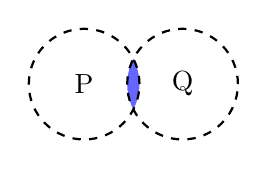
\begin{tikzpicture}
                \begin{scope}
                    \clip (1,1) circle (2em);
                    \fill[blue!60, thick, dashed] (2.25,1) circle (2em);
                \end{scope}
                \draw[black,thick,dashed] (1,1) circle (2em) node {P};
                \draw[black,thick,dashed] (2.25,1) circle (2em) node {Q};
            \end{tikzpicture}
        \end{center}
        Hem de provar que $P\cap Q$ (part blava) és obert. És a dir, hem de provar que $\forall x \in P\cap Q \hbox{ }\exists B_x \subset P\cap Q$,
        on $B_x$ és una bola centrada en un punt $x$ pertanyent a la intersecció.\\
        Com $P$ és obert, $\forall x \in P\hbox{ }\exists B_y^P \subset P$, passa el mateix amb $Q$.\\
        Llavors, $\exists x \in B_x^P \cap B_x^Q \subset P\cap Q$.\\
        Llavors, com $P\cap Q$ té les propietats d'ambdues, és obert.
        \hfill$\square$\\\\
        Ara, provaré que la unió de dos oberts és un obert.
        \begin{center}
            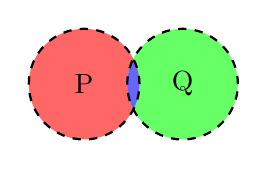
\begin{tikzpicture}
                \fill[red!60,thick,dashed] (1,1) circle (2em) node {P};
                \fill[green!60,thick,dashed] (2.25,1) circle (2em) node {Q};
                \begin{scope}
                    \clip (1,1) circle (2em);
                    \fill[blue!60, thick, dashed] (2.25,1) circle (2em);
                \end{scope}
                \draw[black,thick,dashed] (1,1) circle (2em) node {P};
                \draw[black,thick,dashed] (2.25,1) circle (2em) node {Q};
            \end{tikzpicture}
        \end{center}
        Ens podem adonar fàcilment que un punt qualsevol de $P \cup Q$, pot estar en $P\setminus Q$
        (part vermella), $P\cap Q$ (part blava) o $Q\setminus P$ (part verda). $P\cap Q$ sabem ja
        que és oberta. Tot punt de $P\setminus Q$ està a $P$, i per allò mateix, $P\setminus Q$ és
        obert, anàlogament, tot punt de $Q\setminus P$ està a $Q$, i per allò $P\setminus Q$ és
        obert. Trivialment, podem demostrar que la unió de 2 elements oberts sense cap punt en comú
        segueix sent obert.  
    \end{solucio}

    \setcounter{numex}{7}
    \begin{exercici}
        Descriviu els conjunts de nivell de les funcions següents.
        \begin{itemize}
            \item[h)] 
            \begin{displaymath}
                f\left(x,y,z\right) = x^2 + y^2 + 4y
            \end{displaymath}
        \end{itemize}
    \end{exercici}
    \begin{solucio}
        \begin{obs}
            El valor de $z$ no està al càlcul de la imatge. Per això, en fer l'espai, a l'eix de la 
            $z$ es veurà el generat per $x$ i $y$.
        \end{obs}
        Ens fixem que $f\left(x,y,z\right) = x^2 + \underbrace{y^2 + 4y + 4}_{\left(y+2\right)^2} - 4 = x^2 + \left(y+2\right)^2 - 4$,
        que en conjunts de nivell serà $k+4 = x^2+\left(y+2\right)^2$, és a dir, en fixar $k$ donarà
        una circumferència de centre $\left(0, -2\right)$ i radi $\sqrt{k+4}$. Això fa que no tingui
        sentit $k < -4$, ja que no es pot tindre una circumferència amb radi negatiu (ni l'arrel
        quadrada d'un nombre negatiu està al conjunt dels reals).\\
        Per allò, els conjunts de nivell seran un cilindre de radi $k+4$.\\
        \begin{figure}[h]
            \centering
            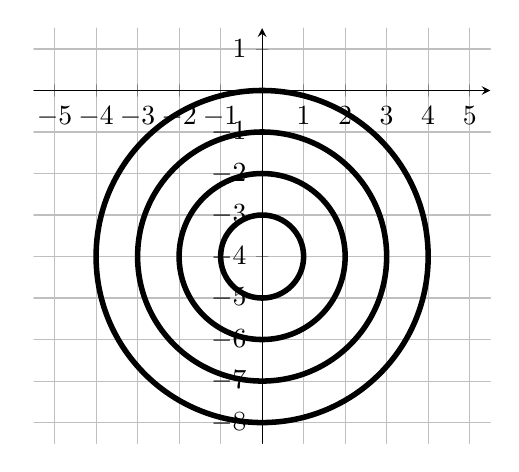
\begin{tikzpicture} [line cap=round,line join=round,>=triangle 45,x=1cm,y=1cm]
                \begin{axis}[
                    x=15pt,y=15pt,
                    axis lines=middle,
                    ymajorgrids=true,
                    xmajorgrids=true,
                    xmin=-5.5,
                    xmax=5.5,
                    ymin=-8.5,
                    ymax=1.5,
                    xtick={-5,-4,...,5},
                    ytick={-8,-7,...,1}
                    ]
                \clip(-7.1428417203702015,-9.767586657202276) rectangle (13.519207331966944,1.643678076075165);
                \draw [line width=2pt] (0,-4) circle (15pt);
                \draw [line width=2pt] (0,-4) circle (30pt);
                \draw [line width=2pt] (0,-4) circle (45pt);
                \draw [line width=2pt] (0,-4) circle (60pt);
                \end{axis}
            \end{tikzpicture}
            \caption{Vista des de $z$}
        \end{figure}
        \\$\hbox{}$
    \end{solucio}

    \setcounter{numex}{10}
    \begin{exercici}
        Calculeu, si existeixen, els límits següents:
        \begin{itemize}
            \item[d)]
            \begin{displaymath}
                \lim\limits_{\left(x,y\right)\rightarrow\left(0,0\right) } \frac{\left(x-y\right)^2}{x^2-y^2}
            \end{displaymath}
        \end{itemize}
    \end{exercici}
    \begin{solucio}
        Primer de tot, provem amb $y = mx$ si depèn de $m$.
        \begin{displaymath}
            \lim\limits_{x\to0} \frac{\left(x-mx\right)^2}{x^2-m^2x^2} = \lim\limits_{x\to0} \frac{x^2\left(1+m^2-2m\right) }{x^2\left(1-m^2\right)} = \frac{1+m^2-2m}{1-m^2}
        \end{displaymath}
        Això, de manera clara, depèn de $m$. Per això no fa falta continuar més. El límit,
        tristament, no existeix.
    \end{solucio}

    \begin{exercici}
        Sigui $f$ la funció definida per
        \begin{displaymath}
            f\left(x,y\right) = 
            \begin{cases}
                \frac{x^2y}{x^2+y^2} & \text{si } \left(x,y\right)  \neq \left(0,0\right)\\
                \alpha & \text{si } \left(x,y\right)  = \left(0,0\right)
            \end{cases} 
        \end{displaymath}
        Decidiu quin valor ha de tenir $\alpha$ per tal que $f$ sigui contínua a tot el pla.
    \end{exercici}
    \begin{solucio}
        Per fer això, hem de trobar $\lim\limits_{\left(x,y\right)\to\left(0,0\right)}\frac{x^2y}{x^2+y^2}$.
        Si aquest límit existeix, aquest límit serà el valor de $\alpha$.
        $\left\lvert \frac{x^2y}{x^2+y^2}\right\rvert = \frac{x^2\left\lvert y\right\rvert}{x^2+y^2}$, sabem que $\frac{x^2}{x^2+y^2} \leq 1$
        llavors tenim $\frac{x^2}{x^2+y^2}\left\lvert y\right\rvert \leq 1\left\lvert y\right\rvert$
        això, quan $y \to 0$ sabem que $=0$. Per allò, $\lim\limits_{\left(x,y\right)\to\left(0,0\right)}\frac{x^2y}{x^2+y^2} = 0$,
        com el límit existeix, $\boxed{\alpha = \lim\limits_{\left(x,y\right)\to\left(0,0\right)}\frac{x^2y}{x^2+y^2} = 0}$
    \end{solucio}
\end{document}